\chapter{Projectmanagement}

\section{Introduction}

\subsubsection*{Purpose of this document}
This chapter shows the project plan for the bachelor thesis "Functional Kafka".
It is used as basis for the planning during the work. 

\subsubsection*{Goal of the project}
Analyzing Apache Kafka, a state of the art message broker system created at
LinkedIn and adapt basic features to build an alternative broker system in
Haskell. 

\section{Organization}

\subsubsection*{Structure}

\begin{tabular}[t]{|l|l|l|} \hline
\textbf{Name} & \textbf{E-mail} & \textbf{Responsibility} \\ \hline
Marc Juchli & mjuchli@hsr.ch & Research, Development, Documentation \\ \hline
Lorenz Wolf & l1wolf@hsr.ch & Research, Development, Documentation \\ \hline 
\end{tabular}

\subsubsection*{Externe Schnittstellen}

\begin{tabular}[t]{|l|l|l|} \hline
\textbf{Name} & \textbf{E-Mail} & \textbf{Responsibility}  \\ \hline
Prof Dr. Josef Joller & jjoller@hsr.ch & Supervisor \\ \hline 
Dr. Simon Meier & simon.y.meier@gmail.com & Expert  \\ \hline\end{tabular}

%\subsubsection*{Sitzungen}

%\begin{itemize}
%\item 
%\end{itemize}

\section{Planning}

\subsection{Time tracking}
Performed work is tracked via Atlassian JIRA platform where we manage issues for
the project. 
%Die Zeiterfassung wird von den Projektmitarbeitern in Redmine erfasst.
%Redmine ist über folgenden Link erreichbar:
%\url{http://152.96.56.42/redmine/}. Die Projektmitarbeiter haben einen
%persönlichen Zugang  um die Daten zu erfassen. Der Betreuer hat
%ebenfalls ein Zugang, mit welchem er die Fortschritte mitverfolgen kann.
%Auf Redmine ist der aktuelle Stand des Projekts zu sehen.

\subsection{Time schedule and objectives}

We separated the work in four phases (adapted from Rational Unified Process,
RUP) as follows:  

\begin{figure}[H]
    \centering
    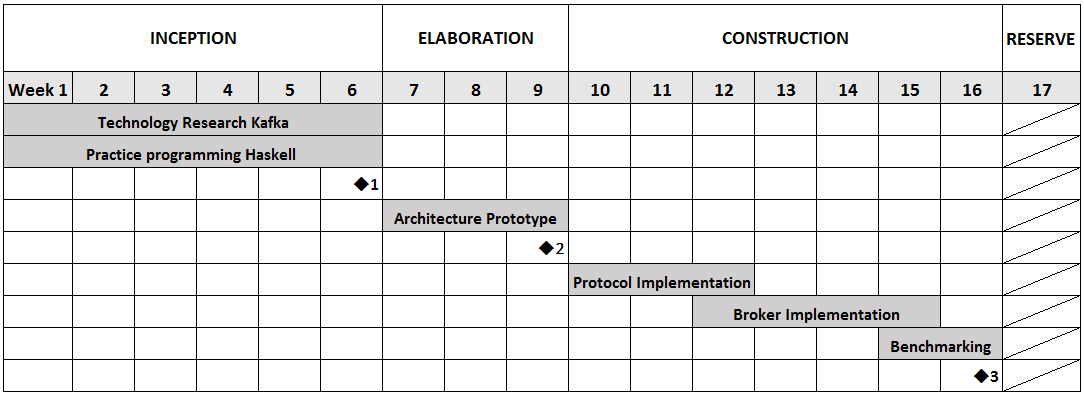
\includegraphics[width=1\textwidth]{images/workschedule.png}
    \caption{Work schedule}
    \label{fig:MBig:the-log}
\end{figure}

\begin{tabular}[H]{|l|l|p{8cm}|}\hline
    \textbf{Phase} & \textbf{Task} & \textbf{Objectives} \\ \hline \hline
    Inception & Technology Research Kafka & 
        \begin {itemize}
            \item Learn Messaging and Event Streaming fundamentals.
            \item Analyse Apache Kafka and related topics. 
            \item Write research documentation.
        \end{itemize} \\ \hline
    Inception & Practice programming Haskell & 
        \begin {itemize}
            \item Familiarize with the functional paradigm.
            \item Setup developer environment and repositories. 
            \item Learn Haskell as functional programming language.
            \item Become acquainted to libraries regarding networking,
              building server application, and serialization.
        \end{itemize} \\ \hline
    Elaboration & Architecture Prototype &
        \begin {itemize}
            \item Set up basic server architecture.
            \item Set up concept for implementing the wire protocol.
            \item Implement basic message workflow from producing messages and
            persisting at broker to consuming the data from another clients.
            \item Implement simplified clients to demonstrate architecture.
        \end{itemize} \\ \hline
    Construction & Protocol Implementation &
        \begin {itemize}
            \item Build standalone package providing an independent Kafka
                protocol library.
            \item Work out details of protocol implementation. Finish
                implementation of relevant parts for producing and consuming
                messages. 
            \item Implement client API for exposing simplified access to protocol
                implementation.
            \item Test Kafka compatibility.
        \end{itemize} \\ \hline
    Construction & Broker Implementation &
        \begin{itemize}
            \item Work out server application handling multiple connections
            sending produce or consume requests.
            \item Develop message log persistency adapt from Apache Kafka. 
            \item Optimize performance to approximate performance approach of
            Apache Kafka. 
        \end{itemize} \\ \hline
    Construction & Benchmarking &
        \begin{itemize}
            \item Test resulting broker implementation for performance.
            \item Comparing performance with Apache Kafka.
        \end{itemize} \\ \hline
    Transition & Reserved & Reserved time for completion work and documentation.
    \\ \hline
\end{tabular}

Important points in the project are specified in table
\ref{tab:MeilensteineZiele}. After reaching the planed end of a milestone, a
set-actual comparison is made. 

\begin{tabular}[t]{|l|l|p{8cm}|}\hline
    \textbf{Milestone} & \textbf{Deadline} & \textbf{Deliverables} \\ \hline \hline
   % M0 & Start of work & 16.02.2015 & - \\ \hline
   % M1 Inception  & 22.03.2015 & 
  %\begin{itemize}
  %  \item \ldots
  %\end{itemize} \\ \hline
\end{tabular}
\captionof{table}{Meilensteine und deren Ziele}
\label{tab:MeilensteineZiele}


\newpage
\section{Risikomanagement(Plagiat)}

In der Tabelle \ref{tab:Risiken} sind die Risiken ersichtlich, welche
unser Projekt beeinflussen können.

\begin{tabular}[t]{|p{3cm}|p{3cm}|r|r|r|p{3cm}|p{3cm}|}\hline
\textbf{Risiko} &
  \textbf{Auswirkung} &
  \begin{sideways} \textbf{Wahrscheinlichkeit } \end{sideways} &
  \begin{sideways}\textbf{Schaden} \end{sideways} &
  \begin{sideways}\textbf{Risiko} \end{sideways} &
  \textbf{Vorbeugung} & \textbf{Konsequenzen} \\ \hline \hline
Datenverlust &
  verlorene Arbeit &
  0.1 & 0.9 & 0.1 &
  regelmässige Backups &
  Arbeit in Sonderschicht nachholen \\ \hline
Ausfall eines Projektmitarbeiters &
  Nichteinhaltung des Terminplans &
  0.1 & 0.9 & 0.1 &
  Nicht vermeidbar &
  Mehrarbeit für nicht ausgefallenen Mitarbeiter \\ \hline
Kommunikations"-probleme &
  Zeitverlust, zielloses Arbeiten &
  0.1 & 0.3 & 0.0 &
  Teambildungs"-massnahmen &
  Diskussion suchen, Betreuer informieren \\ \hline
\end{tabular}
\captionof{table}{Risiken}
\label{tab:Risiken}

Sollte trotz den vorbeugenden Massnahmen ein zeitlicher Schaden
entstehen, muss die Projektplanung unter Umständen angepasst werden.

\section{Qualitätsmanagement}

%Achtungb Plagiat: 
%Um die Arbeitsergebnisse qualitativ auf einem hohen Niveau zu halten,
%arbeiten die Projektmitglieder nach dem Vier-Augen-Prinzip. Ein Dokument
%wird immer von beiden durchgelesen. Allfällige Änderungen werden gleich
%bilateral diskutiert und allenfalls angebracht. Somit soll erreicht
%werden, dass beide Projektmitglieder mit den Ergebnissen einverstanden
%und zufrieden sind.  Um Programmieraufgaben durchzuführen, kann
%teilweise der Ansatz von Pairprogramming eingesetzt werden. Dies führt
%dazu, dass sich beide mit dem Code auskennen.

\section{Projektstandverfolgung}

\subsection{Meilenstein 1}

\section{Zeitauswertung}

\subsection{Projektstunden pro Woche}

\subsection{Projektstunden aufsummiert}

\subsection{Projektstunden pro Projektmitglied}

\subsection{Stunden pro Tätigkeitsbereich}
